\section{CLAS12 Drift Chambers}

The Drift Chambers (DC), which are  part of the large detector system of CLAS12 located in the experimental 
Hall-B at Jefferson Lab. They are used for charged particle detection in the forward direction 
(covering polar angles $5-35^\circ$). The CLAS12 forward detector is built around a six-coil 
toroidal magnet which divides the active detection area into six azimuthal regions, called “sectors”. 
For each sector, there are separate drift chambers installed consisting of 3 regions. Each region contains 
two super-layers, each of them containing 6 layers of wires.   Each layer of the drift chamber 
consists of 112 signal wires making each region a matrix of 12x112. The raw signal from 
one sector makes a matrix of 36x112, which is analyzed independently from other sectors
to extract trajectories of charged particles from raw signals. 

 \begin{figure}[!h]
\begin{center}
 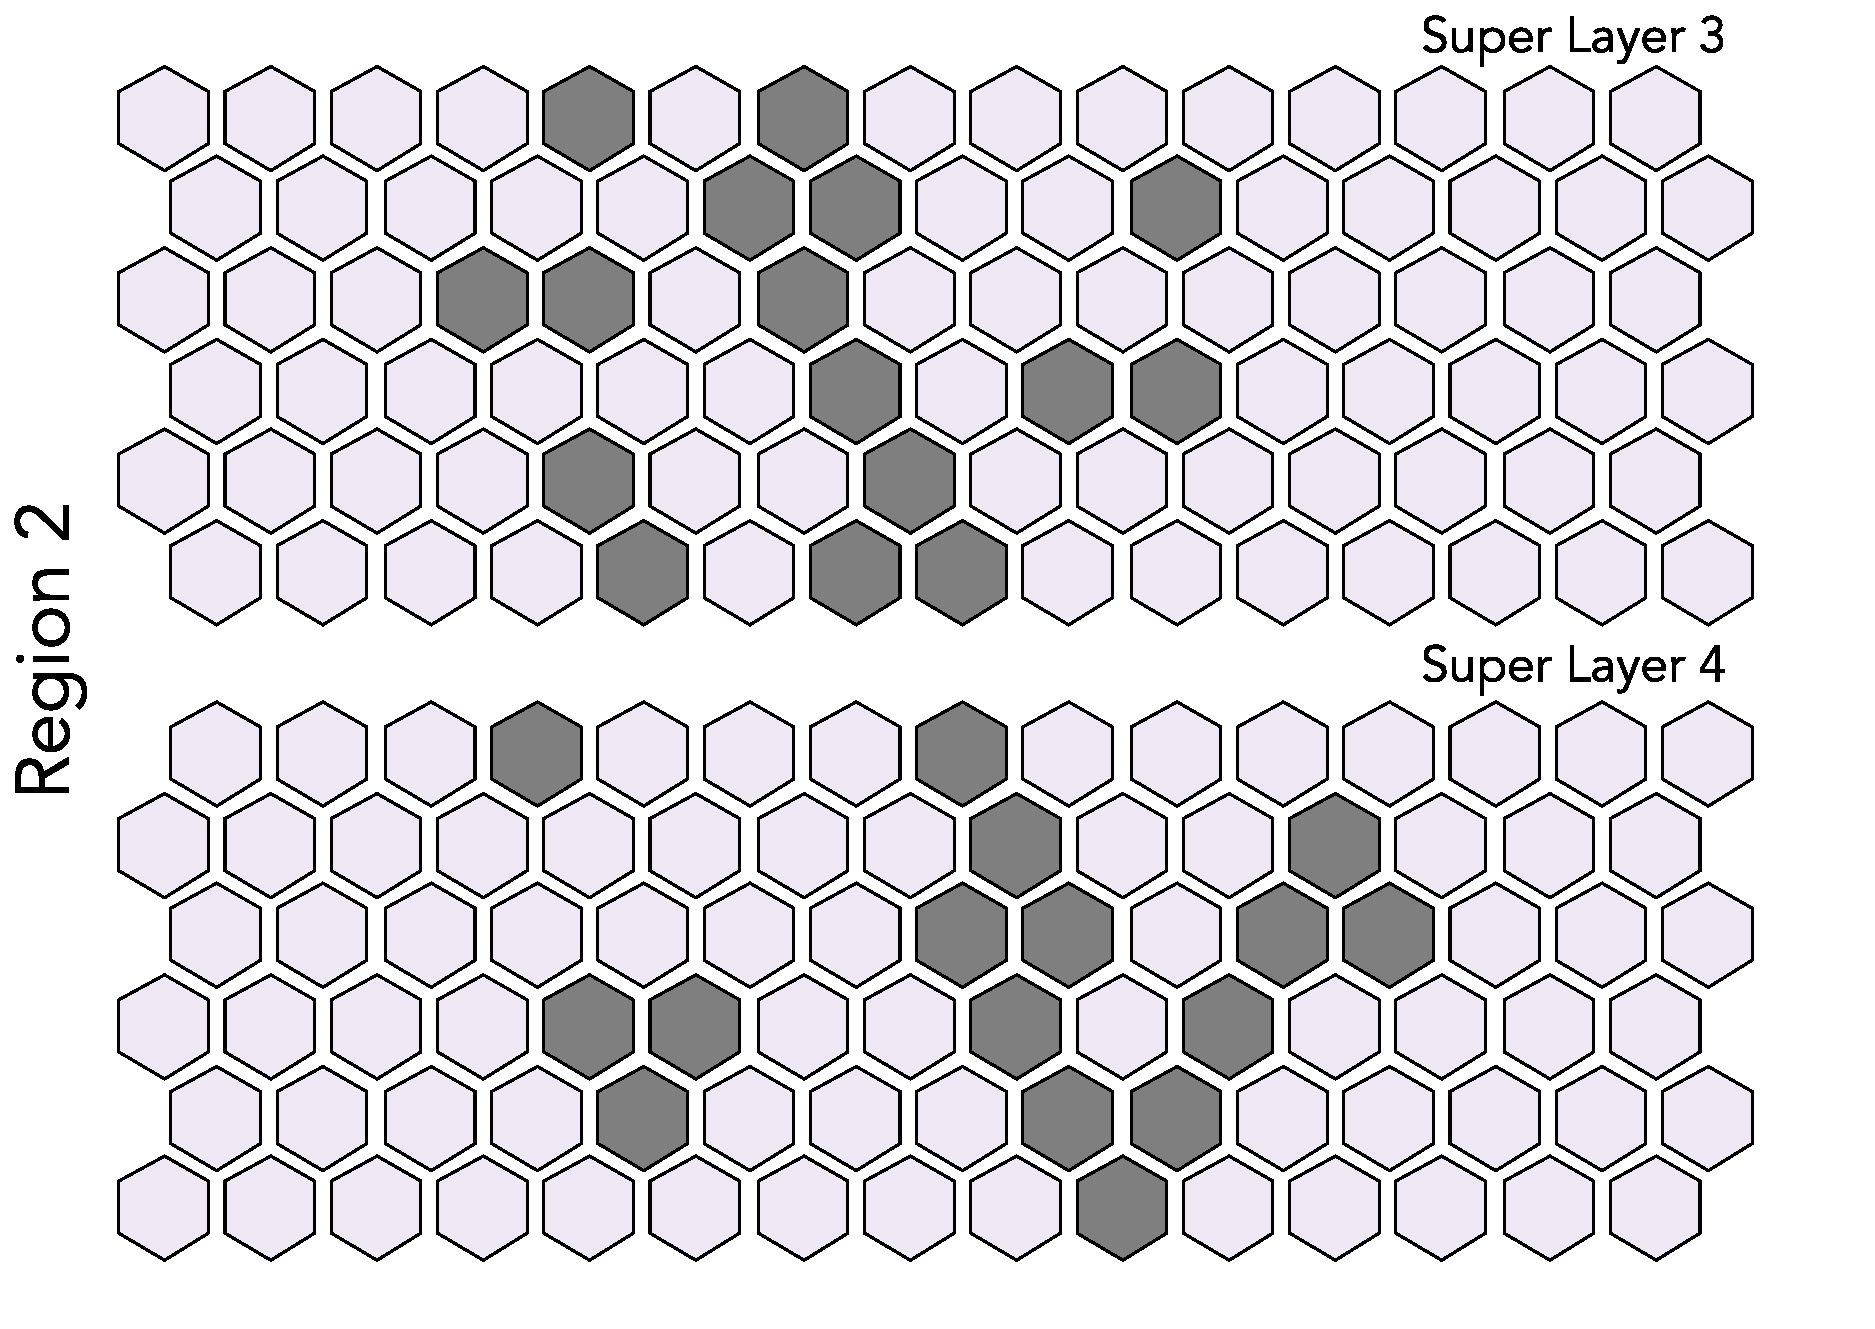
\includegraphics[width=3in]{images/dc_region_2_with_noise.pdf}
 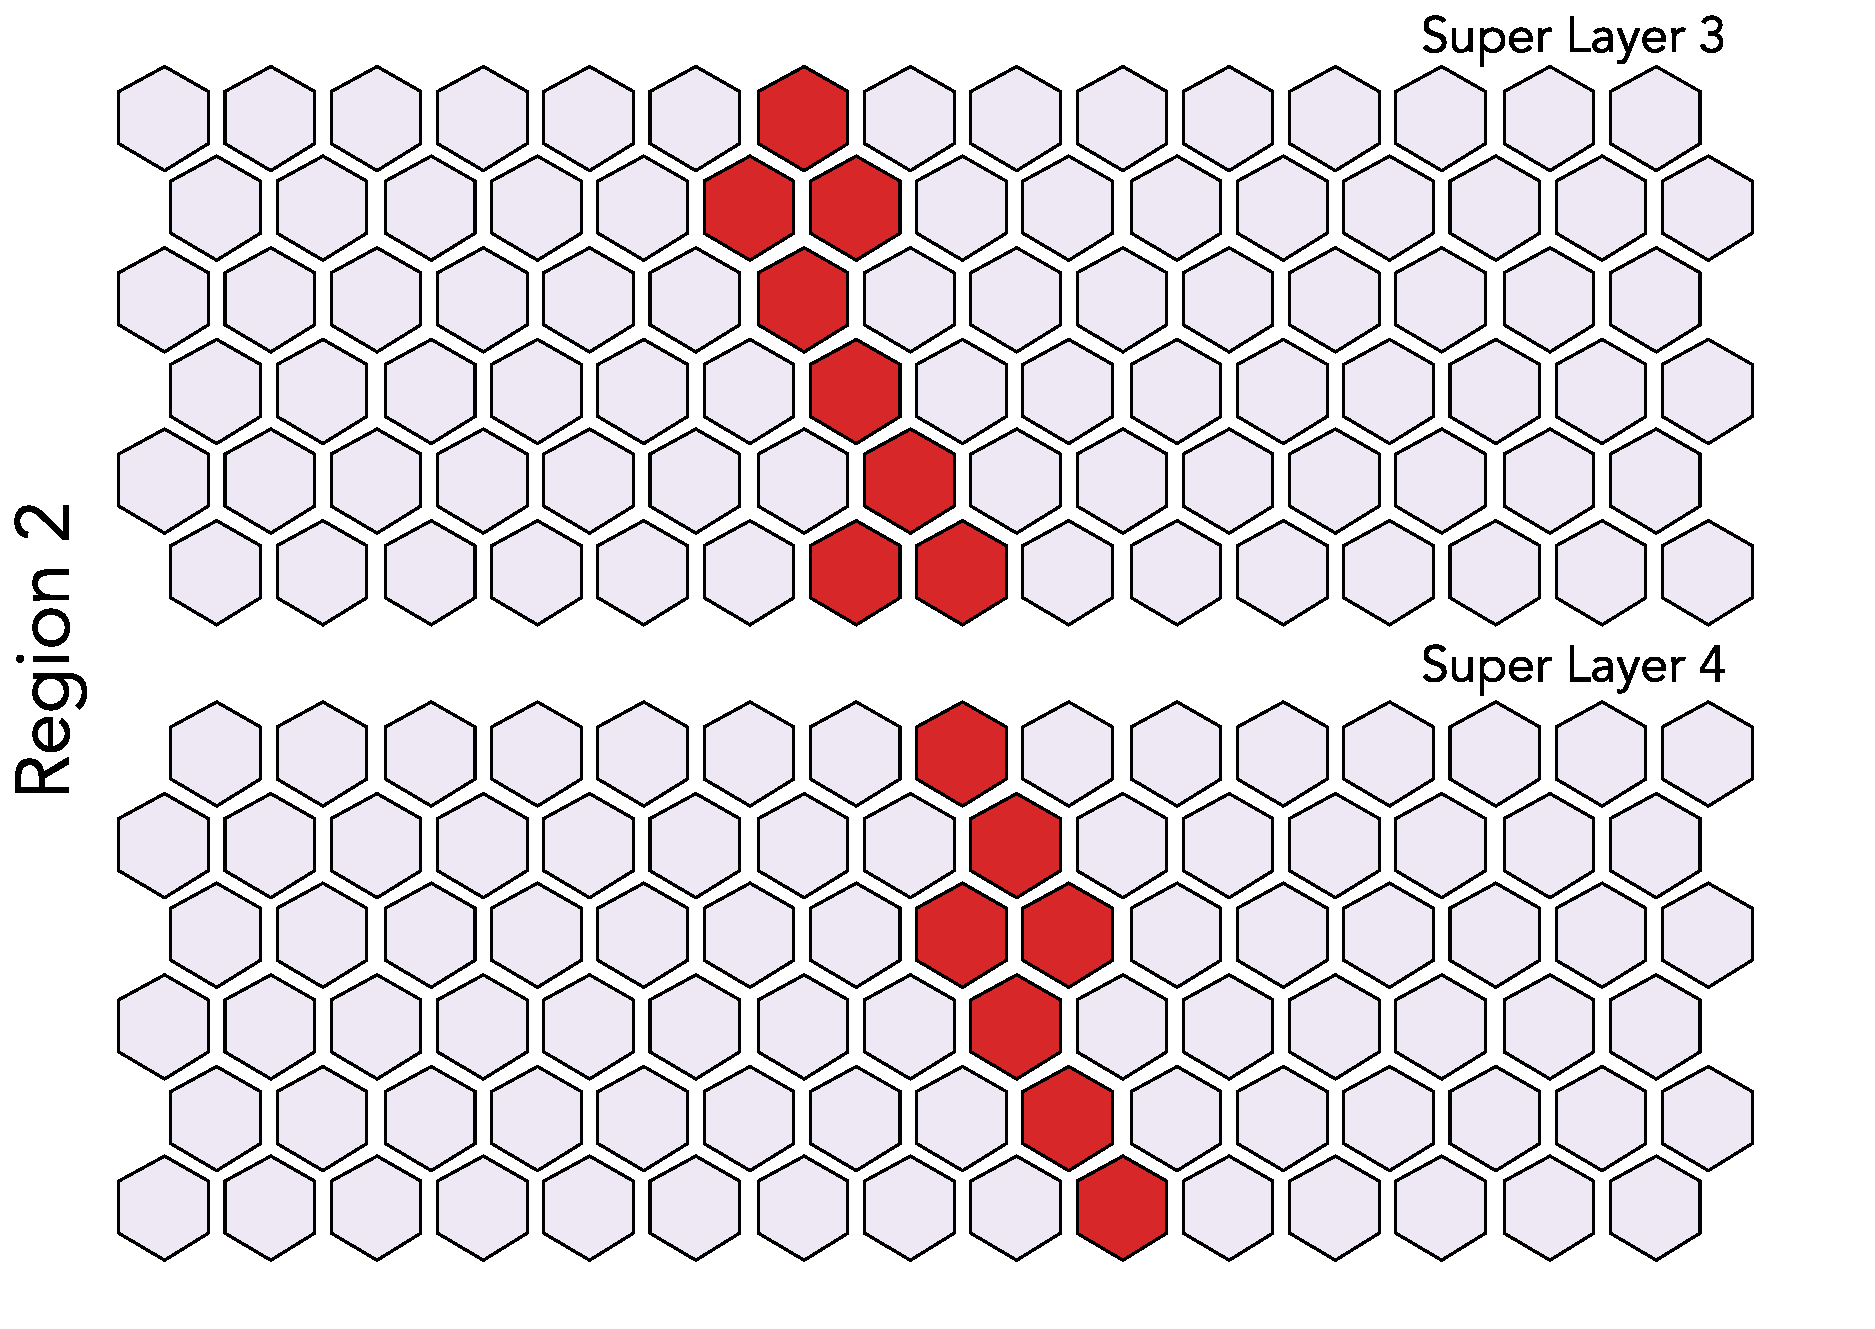
\includegraphics[width=3in]{images/dc_region_2_no_noise.pdf}
\caption {Example of clustering for one region of Drift Chambers. The left panel shows 
all the hits detected in the drift chamber (for this particular region), and the right panel 
shows results of clustering where some hits were identified as a background and were removed,
and the remaining hits were grouped to form a cluster.}
 \label{conv:denoising}
 \end{center}
\end{figure}

Each super-layer is analyzed separately for each sector and hits grouped together along the track trajectory 
are combined into clusters (or segments). In Figure~\ref{conv:denoising} the procedure is shown for one
region where all the hits (dark gray) are shown on the left panel, and clusters (red) are shown on the right panel,
by grouping neighboring wires after removing noise hits. Each super-layer
may have multiple clusters. The tracking algorithm creates a list of track candidates consisting of one cluster 
per super-layer and then analyzes the list to determine which candidates form a valid track. The identified 
tracks are further refined by passing them through Kalman filter~\cite{Kalman1960}. 
Examples of analyzed events in one sector can be seen in Figure~\ref{conv:trackfinding}, where 36x112 matrices
for four sectors are shown (not from the same event) with all signal hits in all layers (top row). The hits 
for clusters for identified tracks are shown on the bottom row. 


 \begin{figure}[!h]
\begin{center}
 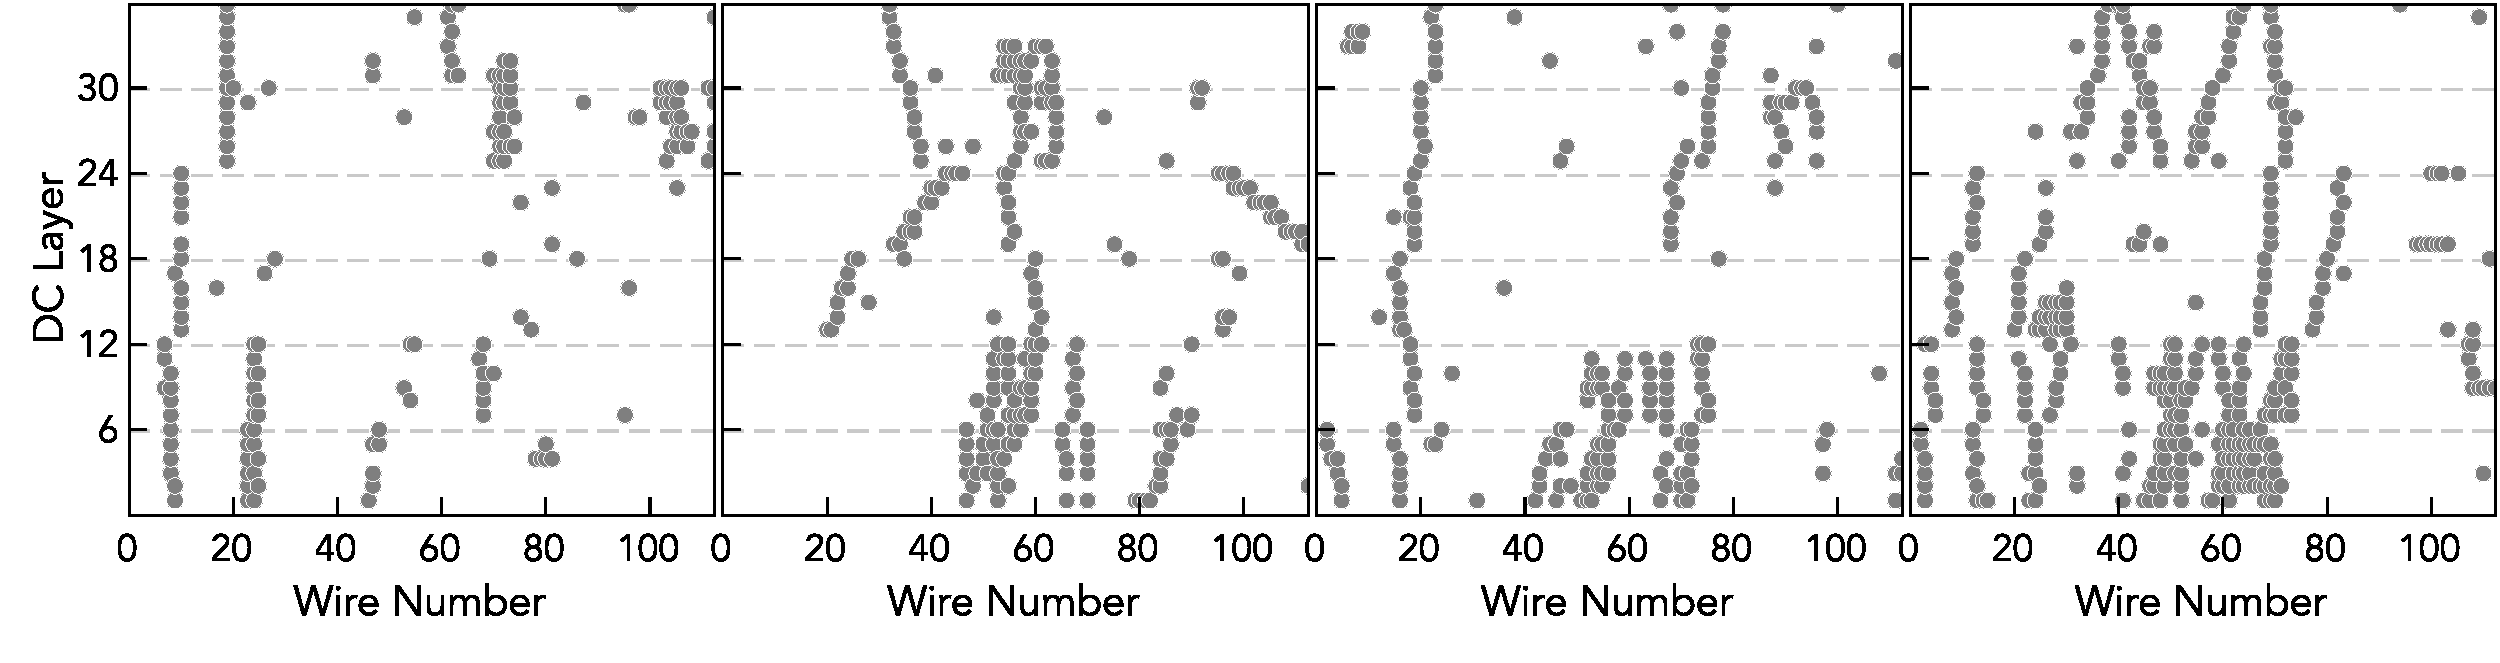
\includegraphics[width=6.0in]{images/dc_example_all_hits.pdf}
 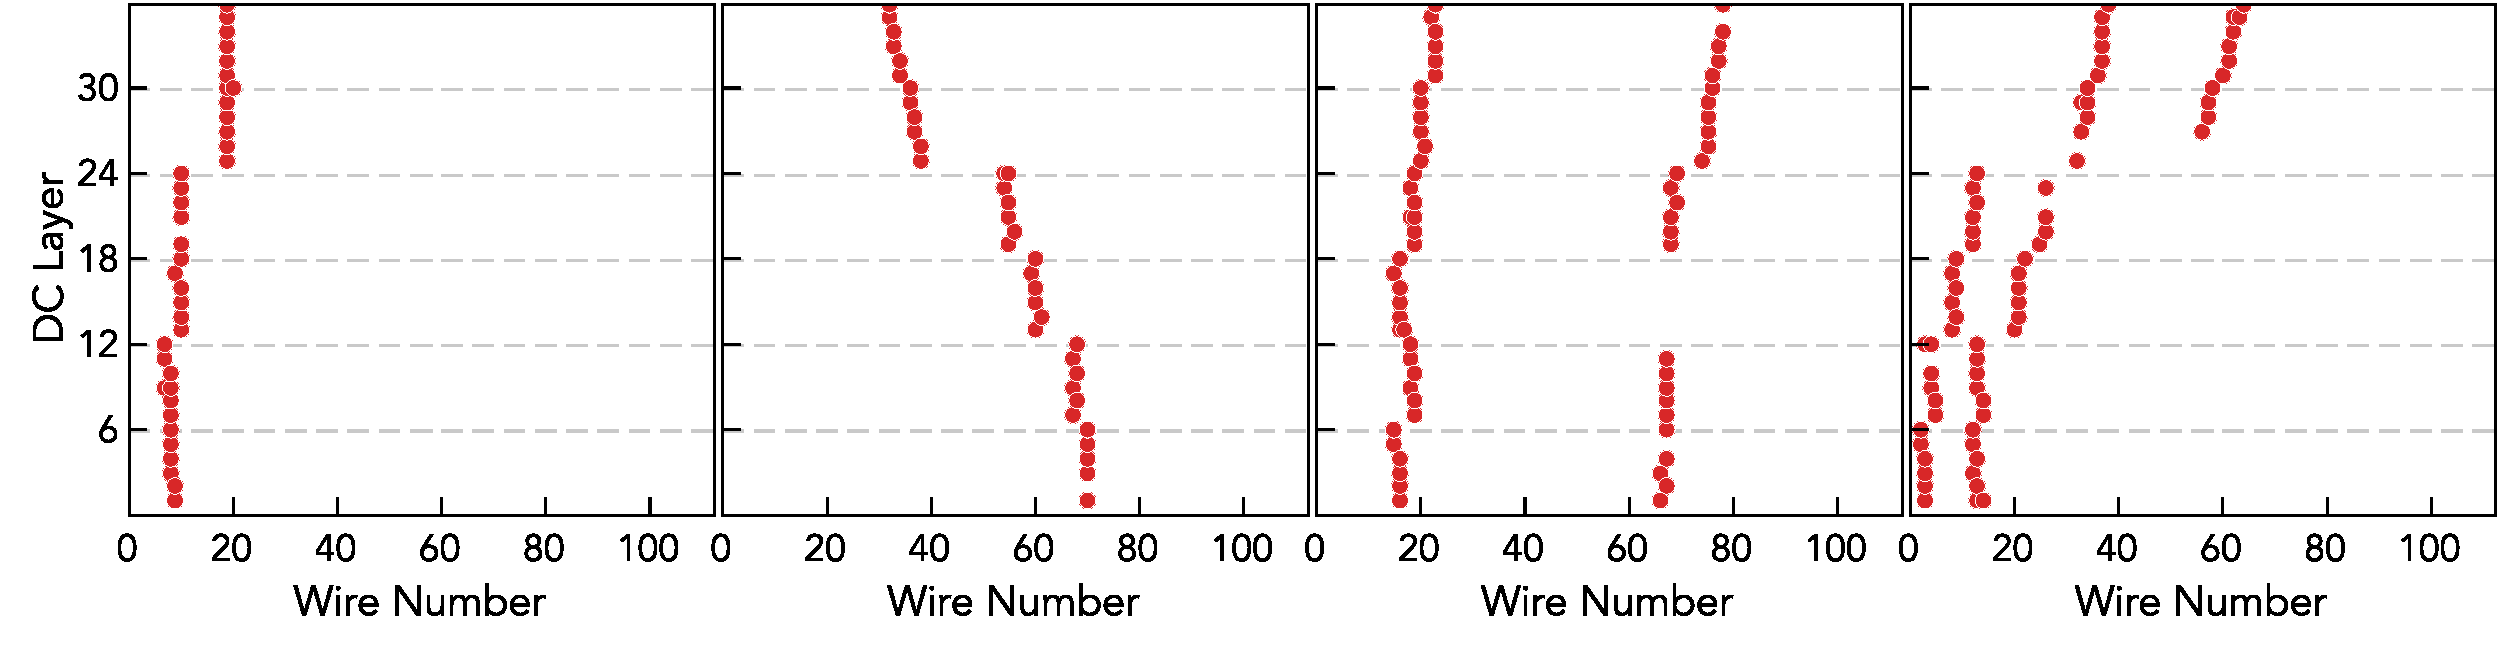
\includegraphics[width=6.0in]{images/dc_example_track_hits.pdf}
\caption {Example of reconstructed tracks in drift chambers. The signal hits in drift chambers are shown 
on the top row. The hits (clusters) belonging to identified tracks are shown on the bottom row. Dashed 
lines represent the boundaries of super-layers.}
 \label{conv:trackfinding}
 \end{center}
\end{figure}

As can be seen from the figure one or multiple tracks can be detected in one sector for the event. The efficiency
of finding these tracks depends on the cluster finding algorithm. With increased luminosity, the number of background 
hits increases, and it becomes difficult to separate background hits from signal hits due to heavy overlap between them.
This results in lost clusters and eventually in a decrease in track finding efficiency. 
In this work, Machine Learning is used to remove background hits prior to the clustering algorithm to improve cluster 
finding and consequentially track finding efficiency. The reconstructed experimental data is used to train Convolutional
Auto-Encoder for de-noising the drift chamber signal~\cite{Thomadakis:2022zcd}.

